%%%%%%%%%%%%%%%%%%%%%%%%%%%%%%%%%%%%%%%%%%%%%%%%%%
% Adam Newton Wright
% Appendix: LGS and Adaptive optics
% app.tex
%%%%%%%%%%%%%%%%%%%%%%%%%%%%%%%%%%%%%%%%%%%%%%%%%%

\appendix

%%%%%%%%%%%%%%%%%%%%%%%%%%%%%%%%%%%%%%%%%%%%%%%%%%
% Laser Guide Stars
%%%%%%%%%%%%%%%%%%%%%%%%%%%%%%%%%%%%%%%%%%%%%%%%%%
\chapter{Laser Guide Stars}

Telescopes observing distant astronomical objects face a significant challenge known as atmospheric distortion. Light coming from these astronomical objects travels in a straight line with little obstruction in the near vacuum of space. However, as a ray of light travels from free space into the atmosphere of Earth, it is affected by the many gaseous particles that make up the atmosphere and result in a different index of refraction than space. The effect is a bending of the light rays, known as \textit{refraction}, that can be described mathematically by Snell's Law, 

\begin{equation}
  n_1 \sin \theta_1 = n_2 \sin \theta_2,
  \label{snellslaw}
\end{equation}
%
where $n_1$ is the index of refraction of the first medium, $n_2$ is the refractive index of the second medium, and $\theta_1$ and $\theta_2$ are the angles that the ray makes with the normal to the interface between the media. A schematic of this is shown in Figure \ref{snellsfigure}.

\begin{figure}[ht!]
  \center
  \includestandalone{Images/tikz/snells}
\caption{Schematic of a ray of light refracting according to Snell's Law as it passes from a medium of refractive index $n_1$ into a medium with higher refractive index $n_2$.}
\label{snellsfigure}
\end{figure}

In general, the many light rays that make up the observed object will be refracted uniformly, causing the object to be perceived in a location that is different from its true position. While that alone is not a problem, if we look closer, we find that the atmosphere does not refract all light rays in the same manner, but small variations in pressure, temperature, and density cause a spatial variation in the index of refraction, resulting in light rays that are close together to be refracted in slightly different ways. This is known as \textit{atmospheric distortion}. A schematic is shown in Figure \ref{fig:atmosphericdistortion}, with plane waves being distorted as they pass through an atmosphere.


\begin{figure}[ht]
  \centering
  \includestandalone{Images/tikz/atmdistortion}
  \caption{Atmospheric distortion of a plane wave passing through Earth's atmosphere}
  \label{fig:atmosphericdistortion}
\end{figure}

The idea of atmospheric distortion will be familiar to those who have seen the sunset on the horizon. As the sun nears the horizon, the light is bent strongly through the atmosphere, resulting in much more distortion than when high in the sky. This results in a disfiguring of its spherical shape and a sharpening around the edges. An example of this is shown in Figure \ref{fig:sunset}.

\begin{figure}[t]
  \centering
  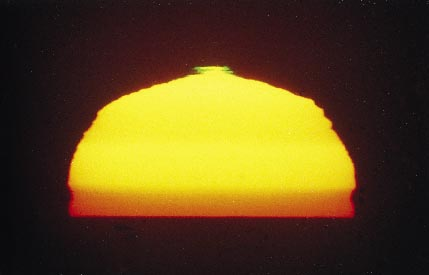
\includegraphics[width = .8\textwidth]{Images/sunset.jpg}
  \caption{Sunset with atmospheric distortion disfiguring the spherical shape of the sun and creating sharp patterns on the edges \protect\cite{sunset}.}
  \label{fig:sunset}
\end{figure}

In order for telescopes to improve resolution, astronomers need to find a way to rid their systems of this atmospheric distortion. One way to do this is to place the telescope outside of Earth's atmosphere where it would be unaffected by atmospheric distortion. This was done with amazing success in 1990 with the low-orbiting, powerful Hubble telescope \cite{Okolski}. However, it is not only extremely costly to put telescopes into orbit, but also impractical as they cannot be easily maintained or serviced.


Thus, a different solution was proposed. If astronomers could model how light was distorted as it passed through the atmosphere, they could subtract those distortions from their images and obtain higher resolution data. In order to measure the amount of distortion present, telescopes can observe a point source in the sky, such as a distant star, and observe its image. This image is then compared with the image of an ideal point source not affected by atmospheric distortion, and the difference between these two images represents the amount of distortion. Once the distortion is known, it is sent to a deformable mirror, which is made of many smaller mirrors, each able to move independently from the others. The deformable mirror can then create a wavefront conjugate to the distortion calculated. By reflecting the image of astronomical object off this mirror, the distortion is removed from the image. This process is known as \textit{adaptive optics}, and more information is given in Appendix B.


However, there are not always stars bright enough in the telescope's field of view that can be used as this point source (better known as  guide star) \cite{Wizinowich2006}. In order to skirt this problem, artificial stars were constructed, known as \textit{laser guide stars} (LGS). A laser guide star is created by sending laser light into the atmosphere, where it interacts with a layer of sodium atoms. These sodium atoms reside approximately $\SI{60}{\kilo\meter}$ from Earth in a $\SI{10}{\kilo\meter}$ thick layer of the atmosphere known as the mesosphere. A figure of this region within the layers of Earth's atmosphere is shown in Figure \ref{fig:mesosphere}. These atoms are deposited from meteors as they burn up in Earth's atmosphere, leaving behind their composite particles, a significant portion being sodium. The density of this sodium layer varies throughout a given day and throughout the year, but typically is near $\SI{5e13}{atoms \per \meter \cubed}$ \cite{Kibblewhite2009}. Using a laser with a wavelength resonant with sodium,  the atoms will absorb and emit this light, creating a glowing sphere in the upper atmosphere, as mentioned in Chapter 2. This sphere of light is then used as the guide star.\footnote{There are actually two types of laser guide stars: sodium based and Rayleigh scattering based. Rayleigh scattering laser guide stars rely on the scattering of light in the atmosphere, as opposed to having atoms absorb and emit light.}

\begin{figure}
		\center
		\includestandalone{Images/tikz/mesosphere}
	\caption{Schematic of sodium atoms residing in the mesosphere.}
	\label{fig:mesosphere}
\end{figure}



In general, most large-scale, ground-based telescopes now have powerful lasers with wavelengths precisely tuned to be resonant with sodium. As these telescopes are making observations, the lasers are shone into the sky to create the LGS. An image of an LGS being created is shown in Figure \ref{fig:LGSatESO}. The LGS is observed and atmospheric distortions are calculated and subtracted from the image in real time.

\begin{figure}[hb!]
  \centering
  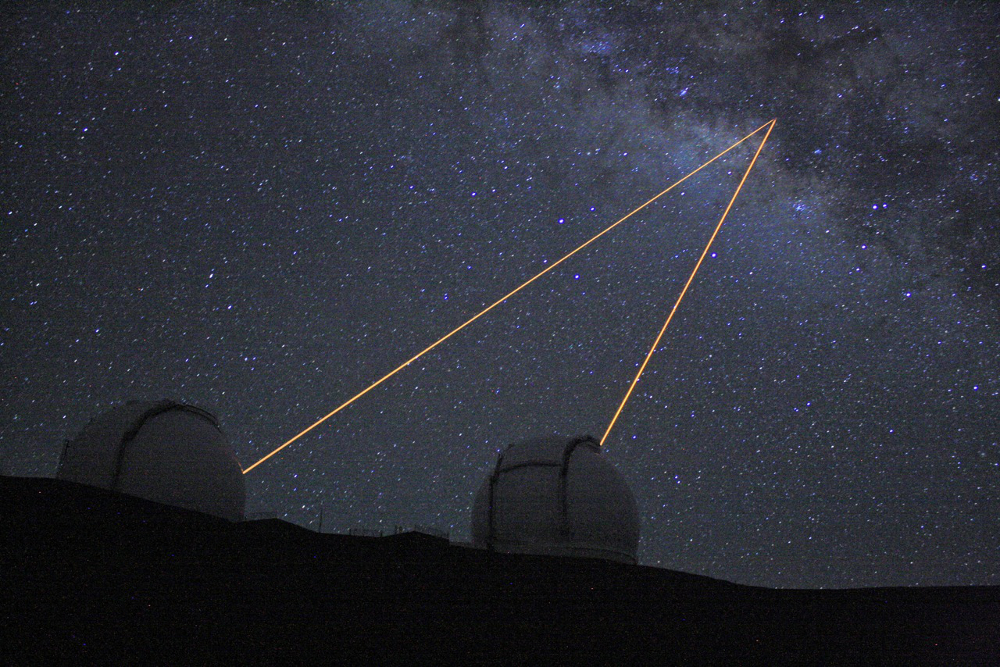
\includegraphics[width = .8\textwidth]{Images/LGSatESO.jpg}
  \caption{Laser guide star being created at the Very Large Telescope \protect\cite{VLT}.}
  \label{fig:LGSatESO}
\end{figure}

One major concern for LGS systems is their brightness in the sky \cite{Wizinowich2006}. It is important for the star to be bright enough that the telescope system is able to pick up enough light for a measurement of the distortion. The shape of the LGS is also important, as it must be as near to circular as possible in order for an accurate measurement of the distortion to be made. The shape of the LGS is mostly due to the profile of the laser beam \cite{Holzlohner2012} and will not be discussed here.

In order to create a brighter laser guide star, a few methods are utilized. One method is to increase the intensity, the power per unit area, of the laser. Typical laser intensities are of the order of \SI{20}{W \per \meter \squared} \cite{Kane2014}. This allows for more atoms to absorb and emit light, thereby creating a brighter star. Another method is to increase the diameter of the laser beam, which will allow for a greater area of sodium atoms to be reached by the light. These both have limitations, however. The power cannot continually be increased because of limitations on the power of lasers and due to downpumping \cite{Kane2014}. The size of the LGS also should not be continually increased since, for adaptive optics to work, the assumption is made that the LGS is a point source. A more sophisticated method, optical pumping (discussed in Chapter 2), makes use of circularly polarized light to move the atom into a cycling transition. The method explored in this thesis expounds on using circularly polarized light, but realizes the effects of the geomagnetic field on the distribution of angular momentum when circularly polarized light is used, and uses a pulsed laser to counteract this.


%%%%%%%%%%%%%%%%%%%%%%%%%%%%%%%%%%%%%%%%%%%%%%%%%%
% Adaptive Optics
%%%%%%%%%%%%%%%%%%%%%%%%%%%%%%%%%%%%%%%%%%%%%%%%%%

\chapter{Adaptive Optics}
The process of measuring the atmospheric distortion in order to enhance astronomical imaging, known as \textit{adaptive optics}, is a mathematical estimation problem. Here, we present an introduction to the methods used during this process.

In general, telescopes observe the LGS and the astronomical object simultaneously. The image of the LGS is then compared to an ideal point source imaged through the telescope without atmospheric distortion,\footnote{This is typically done using optical modelling software, but can also be done experimentally using various quasi-pointlike source objects.} and the distortion is calculated by comparing the two. A deformable mirror, composed of many smaller mirrors each of which can be moved independently of the others, is then used to create the opposite of the calculated distortion. The image of the astronomical object is then reflected off this mirror, thereby ridding the image of distortion.

In order to calculate the atmospheric distortion, astronomers make use of the well defined way in which point sources are imaged through optical systems. When an idealized point in object space is imaged through an optical system, it has a certain energy distribution in image space, known as the point spread function. For an optical system with spherical symmetry and no aberration, the point spread function can be described mathematically along the radial coordinate $x$ as

\begin{equation}
  P(x) = \frac{J_1(x)}{x},
  \label{psfa}
\end{equation}
%
where $J_1(x)$ is the Bessel function of the first kind. This function is known as the \textit{Airy disk}, and is shown in Figure \ref{fig:airydiska}. It is an idealized description of a point imaged through a perfect optical system.

%\begin{figure}[h]
%  \centering
%  \begin{tikzpicture}
%	\begin{axis}
%	  \addplot3[surf,z buffer=sort,domain=-5:5,y domain=-5:5] gnuplot {airy((x**2+y**2)**(1/2))};
%	\end{axis}
%\end{tikzpicture}
%  \caption{<+caption text+>}
%  \label{fig:<+label+>}
%\end{figure}<++>




\begin{figure}[h]
  \centering
  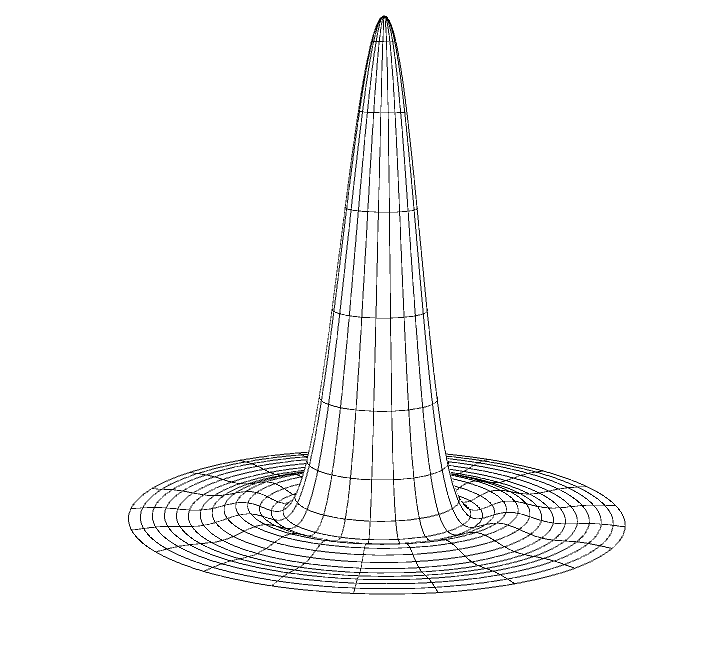
\includegraphics[scale = .4]{Images/airydisk.png}
  \caption{Graph of the Airy disk function, describing an idealized point imaged through a spherically symmetric, aberration free optical system.}
  \label{fig:airydiska}
\end{figure}

It turns out that stars are very close to being point sources and can thus be used as this idealized point source. Since the light from these stars is passing through Earth's atmosphere, it will be distorted, and these distortions will show up in the point spread function, thus deviating from the Airy Disk described by Equation \ref{psfa}. 

Astronomers then use a combination of Fourier mathematics and an optimization algorithm to calculate the distortion. This method follows that outlined by Gonsalves \cite{Gonsalves1982}. This is done by first calculating optical transfer function

\begin{equation}
  H(\omega) = A(\omega) e^{i \theta(\omega)},
  \label{opticaltransfera}
\end{equation}
%
where $A(\omega)$ is the Fourier transform of the aperture function\footnote{The aperture function is a function describing where light can and cannot pass through. For a circular aperture, it would consist of a solid circle where light can pass through and nothing around the circle. It essentially acts like the computational version of a camera aperture.} of the system and $\theta(\omega)$ is the phase of the incoming light. The phase of the light can be described as a summation,

\begin{equation}
  \theta (\omega) = \sum _{k=0} ^{\infty} c_k \phi (\omega),
  \label{phasesuma}
\end{equation}
%
where $\{\phi (\omega) \}$ is a set of polynomials\footnote{The idea of using a set of polynomials to described the phase is similar to the idea of using sinusoidal functions in Fourier analysis to deconstruct a signal.} and $c_k$ is a coefficient that quantifies how much of each polynomial is present in the distortion. Taking the inverse Fourier transform and then the modulus squared, we can calculate the point spread function of this light

\begin{equation}
		P(x) = \Big|\text{ifft}[H(\omega)]\Big|^2,
  \label{otftopsfa}
\end{equation}
%
where $\text{ifft}$ denotes the inverse Fourier transform of the argument. This method allows us to mathematically create a point spread function simply by estimating the phase of the light with a set of polynomials.

Using this method, we have a way to estimate the distortion present in an image. First, a set of polynomials is selected. A possible set of polynomials to use is the Zernike set \cite{Gonsalves1982},\footnote{The Zernike set of polynomials described many optical distortions such as spherical aberration, defocus, coma, etc., and is chosen for systems displaying these distortions} but there are many others that can be used. Second, a coefficient list, or ``vector,'' of numbers is created in which each number will be the coefficient in front of its corresponding polynomial in the set of polynomials. This gives us a way to weight each of the polynomials in the set. Next, an algorithm is set up to change each number in the coefficient list, and, at each change, the point spread function is calculated (by the method above). This calculated, or estimated, point spread function is then compared to the observed point spread function, and an error metric is calculated. The algorithm will seek to minimize this error metric. Once this is minimized, the calculated point spread will be quite similar to the observed point spread function, and, at this point, we know the distortion acting on the system. The distortion is simply the set of polynomials, each weighted by its coefficient found by the algorithm.


Searching for the correct polynomials weighted by the correct coefficients is not trivial. Sometimes certain polynomials can be ignored if it is known by symmetry that they will not show up in the point spread function. Regardless, searching for the correct distortion is an optimization of a function in a large parameter space. Typical algorithms use a steepest descent approach \cite{Gonsalves1982}, which changes one parameter at a time, calculates an error between that estimation and the observed point spread function, and seeks to minimize this error. There have also been algorithms that use random searches, Monte Carlo walks, and Markov chain Monte Carlo searches that claim robustness and speed \cite{fienup}.

Once the correct distortion is calculated, the information is sent to the deformable mirror. This mirror consists of many smaller mirrors, each of which can be precisely adjusted by a piezoelectric actuator. The mirror changes shape, or adapts to the distortion,\footnote{This is where the term ``adaptive optics'' comes from.} creating a conjugate wavefront that the image from the telescope can be reflected off. At this point, the atmospheric distortion has been removed from the image. Normally, this is done in real time, and thus speed of both the calculation algorithm and of the movement of the deformable mirror must be optimized. Systems typically can calculate and adjust in under a second \cite{Wizinowich2006}.


%\begin{equation}
%  \begin{split}
%	Z_n^m (\rho,\phi) &= R_n^m (\rho) \cos(m\phi)\\
%	Z_n^{-m} (\rho, \phi) & = R_n^m (\rho) \sin(m\phi)\\
%	R_n^m (\rho) & = \sum _{k=0} ^{\frac{n-m}{2}} \frac{(-1)^k (n-k)!}{k!(\frac{n+m}{2}-k)! (\frac{n-m}{2}+k)}
%  \end{split}
%  \label{zernike}
%\end{equation}


